{\fontsize{12pt}{22pt} \textbf{Non-Parametric Tests}\par}

\vspace{5mm}

Example 1 \textbf{(Kolmogorov-Smirnov test)}: 

\vspace{5mm}

- Test whether a sample follow a known law \\

$F$ is the cumulative ditribution function and $\widehat{F_n}$ its empirical estimation. \\

The statistic test is $\widehat{F_n}(x) - F(x)$. \\

We have, \\

$\sqrt{n} \underset{1 \leq i \leq k}{\operatorname{max}}|\widehat{F_n}(x_i) - F(x_i)| \underset{n \rightarrow + \infty}{\rightarrow} \underset{0 \leq i \leq k}{\operatorname{max}}|W_i|$ where $W_i$ is a \textit{Brownian motion} or \textit{Wiener process}.\\

We also have, \\

$\sqrt{n} \underset{0 \leq x \leq 1}{\operatorname{max}}|\widehat{F_n}(x) -x)| \underset{n \rightarrow + \infty}{\rightarrow} \underset{0 \leq x \leq 1}{\operatorname{max}}|B(x)|$ where $B$ is a \textit{Brownian bridge}.\\

\href{http://www.math.utah.edu/~davar/ps-pdf-files/Kolmogorov-Smirnov.pdf}{Proofs (Empirical-Process Theory)} \\

A Brownian bridge has the following property: \\

$\mathbb{P}(\underset{t \in [0,1]}{\operatorname{sup}}|B_t| \geq b) = 2 \Sigma_{n \geq 1}(-1)^{n-1}e^{-2n^2b^2}$.

This allowed statisticians to draw a quantile table, we can thus easily know the critical region.

\vspace{5mm}

- Test whether two samples follow the same law \\

In that case, the statistic is the distance $D_{n,m} = sup_x |\widehat{F}_{1,n}(x) - \widehat{F}_{2,m}(x)|$. \\

Associated test hypothesis are: \\

$
\left\{
    \begin{array}{ll}
        \mathcal{H}_0: \widehat{F}_{1,n}(x) = \widehat{F}_{2,m}(x) \\
        \mathcal{H}_1: \widehat{F}_{1,n}(x) \neq \widehat{F}_{2,m}(x) \\
    \end{array}
\right.
$

We reject the null hypothesis for level $\alpha$ if $D_{n,m} > \frac{1}{\sqrt{n}} \sqrt{-ln(\frac{\alpha}{2}) \frac{1 + \frac{n}{m}}{2}}$. \\

\textit{Scipy} \\

\underline{Test statistic computation}

\lstset{language=Python}
\lstset{frame=lines}
\lstset{caption={Kolmogorov-Smirnov test statistic}}
\lstset{label={lst:code_direct}}
\lstset{basicstyle=\footnotesize}
\begin{lstlisting}

cdf1 = np.searchsorted(data1, data_all, side='right') / n1
cdf2 = np.searchsorted(data2, data_all, side='right') / n2
cddiffs = cdf1 - cdf2
T = np.max(cddiffs)

\end{lstlisting}

\underline{Critical probability computation} \\

The critical probability is computed differently depending on sample size. If sample size is small, an exact computation is done. If sample size is large, an asymptotic computation is done.
In both cases, the critical probability is computed using combinatorics and largely inspired by \href{https://projecteuclid.org/download/pdf_1/euclid.afm/1485893310}{J. L. Hodges, Jr.}.

\vspace{5mm}

Example 2 \textbf{(Wilcoxon-Mann-Whitney test} or \textbf{Mann-Whitney U test)}: 

\vspace{5mm}

- Test whether two samples follow the same law \\

$
\left\{
    \begin{array}{ll}
        \mathcal{H}_0: \widehat{F}_{1,n}(x) = \widehat{F}_{2,m}(x) \\
        \mathcal{H}_1: \widehat{F}_{1,n}(x) \neq \widehat{F}_{2,m}(x) \\
    \end{array}
\right.
$

\vspace{5mm}

The test statistic is $U = \Sigma rank_1 - \frac{n_1(n_1+1)}{2}$ where $rank_1$ are the ranks of each element from the first dataset in the second dataset. \\

\underline{Intuition behind the test}

The test is equivalent of ranking all elements from the two datasets; if the resulting dataset is well mixed, the p-value is likely to be high (similar distributions).

The test can also be interpreted as a comparison between the two medians; if they are very different, distributions are likely to be different.

\vspace{5mm}

Example 3 \textbf{(Fisher exact test)}: 

\vspace{5mm}

- Test whether proportions are representative \\

$\mathcal{H}_0: \text{proportions are representative} $ \\

This test is to be used for the analysis of contingency tables.

\begin{center}
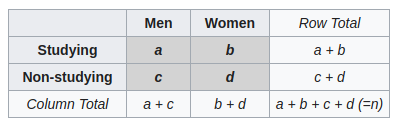
\includegraphics[scale=0.6]{fisher_contingency_table.png}
\end{center}

Fisher showed that knowing the total numbers (Row Total and Column Total), the probability to have a certain combination follows a \textit{hypergeometric} distribution.

$$p = \frac{C_a^{a+b} C_c^{c+d}}{C_{a+c}^n}$$

The test is said \textit{exact} since there is no asymptotic behavior in the formula. \\

$p < \alpha$ means that, based on total numbers, this specific combination is unlikely to happen.

\vspace{5mm}